\section{OpenCV \texttt{THRESH\_TRIANGLE}}
%Refenz ???
The OpenCV function \texttt{cv2.threshold()} can be used to binary threshold an image with different methods \cite{cv_thresh}.

Since the method \texttt{THRESH\_TRIANGLE} is not very well described in the OpenCV documentation, a small explanation of it is provided here. First the function builds the histogram of the given image. Next it searches for the highest point and the first values from the border left and right which are not zero. Then it compares the distance between the position of the highest point and the position of the first non zero points left and right. The point with the bigger distance is used as an corner point for a triangle. The triangle can be seen in the Figure \ref{theory:triangle}.
\begin{figure}[ht]
	\centering
	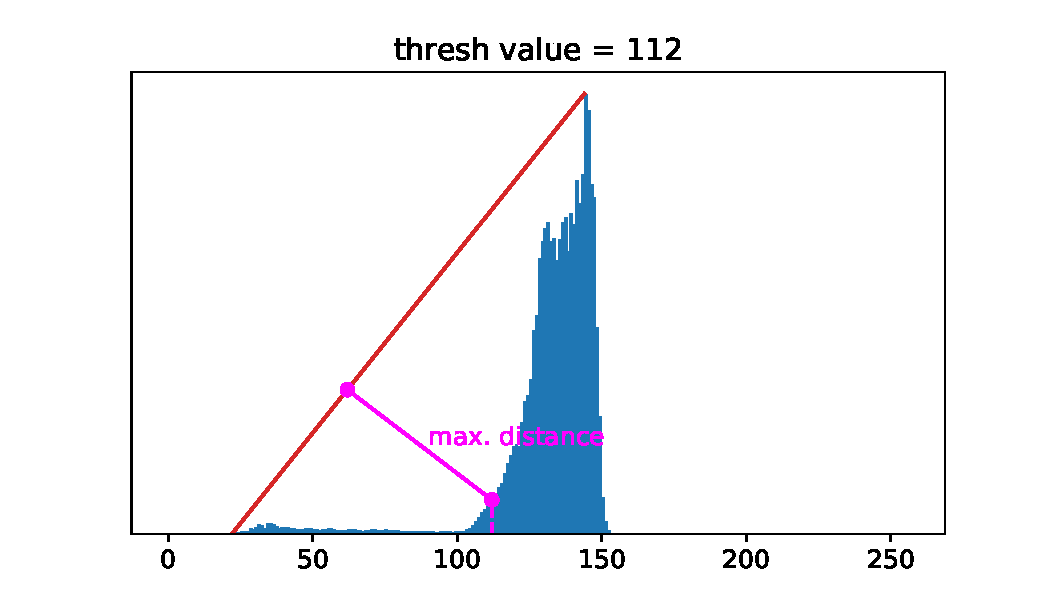
\includegraphics[width=0.9\textwidth]{2-theory/threshold/triangle.pdf}
	\caption{Threshold triangle shown in histogram.\label{theory:triangle}}
\end{figure} 
The hypotenuse of the triangle is now used to find orthogonal line between the hypotenuse and the histogram. To find this, usually all distance values have to be calculated. To find the correct length between the histogram and the hypotenuse, there is some complex geometry involved which is time consuming. To make the algorithm faster, OpenCV makes an approximation. To better understand what is calculated we look at the OpenCV C++ code in Figure \ref{theory:code} which implements the triangle threshold. 

\definecolor{codegreen}{rgb}{0,0.6,0}
\definecolor{codegray}{rgb}{0.5,0.5,0.5}
\definecolor{codepurple}{rgb}{0.8,0,0.82}
\definecolor{backcolour}{rgb}{0.95,0.95,0.92}
\definecolor{dred}{rgb}{0.7,0,0}

\lstdefinestyle{mystyle}{
	backgroundcolor=\color{backcolour},   
	commentstyle=\color{codegreen},
	keywordstyle=\color{dred},
	numberstyle=\tiny\color{white},
	stringstyle=\color{codepurple},
	basicstyle=\footnotesize\ttfamily,
	breakatwhitespace=false,         
	breaklines=true,                 
	captionpos=b,                    
	keepspaces=true,                 
	numbers=left,                    
	numbersep=2pt,                  
	showspaces=false,                
	showstringspaces=false,
	showtabs=false,                  
	tabsize=2
}
\lstset{style=mystyle}
\lstdefinestyle{mystyle}{
	morekeywords={cwt,contourf,datetick}
} 
\begin{figure}[ht]
	\centering
	\lstinputlisting[language=C++,firstline=1301,lastline=1310,numbers=left,style = mystyle]{2-theory/threshold/thresh.cpp}
	\caption{C++ code snipped \cite{cv_code}.}
	\label{theory:code}
\end{figure}
In the line one we have our max height a and the distance between left border and the place where a is located. The histogram is saved in the array h with 256 places, where the place itself represents the brightness value from zero to 255.\\
To keep the algorithm fast the author of this code snipped decided that an approximation to find the biggest distance between the hypotenuse and the histogram is good enough. To obtain the biggest distance the max value a gets multiplied with the index i and added together with b multiplied by the histogram value at the index i. The result of this calculation gets temporary saved. This process is now repeated for all values in between b and the index of a. If the new calculation is bigger the value and the index are saved. With this the algorithm saves the index where the biggest distance occurs. The function itself only returns the index itself which is saved in the variable tresh. \\
With this tresh value a normal binary threshold is processed over the given image. Resulting in a one and zero image.   
\newpage